\chapter{Methods for implementation}\label{cha:method_implementation}
This chapter gives a detailed description of the methods used for solving the problem formulations of this thesis. The chapter is divided into two different parts. The first part gives a detailed description about the implementation of the distance transform module. This part has been reimplemented several times due to poor performance of the used methods. The second part gives a detailed description about the implementation of the distance field rendering module.

\section{Distance field generation initial attempt}
It exists many EDT algorithms for creating distance fields. Most of the EDT algorithms used today runs in $\mathcal{O}(nm)$, where n and m are the width respectively the height of the image. Example of algorithms running in $\mathcal{O}(nm)$ are \citet{Danielsson} and \citet{meijster}.

The initial implementation of distance field generation in this thesis was built around \citet{Gustavson:2011} article on the subject. A signed version of the 8SED algorithm was used along with the anti-aliased sub-pixel distance measure proposed in the article. A signed distance field has several advantages compared to an unsigned distance field. The most obvious advantages is the increased flexibility it gives and that it facilitates the implementation of proper anti-aliasing around the border of the shape\citep{gustavson20122d}. To generate a signed distance field the distance transform was run twice with inverted input representation. The first transforms creates a distance field on the inside of the glyph and the second transform on the outside of the glyph. The resulting distance field was then calculated with the following formula.\vspace{\baselineskip}\newline
$result(i,j) = inside(i,j) - outside(i,j), \forall (i, j), i \in \{0,\dots, m-1\}, j \in \{0,\dots, n-1\}$ \vspace{\baselineskip}\newline
\section{Fast and approximate distance field generation}
Fast distance field generation on mobile devices requires some approximations and optimizations to decrease the transformation time. This can be seen in many of the of the distance field generation implementations done lately. Two examples of this is GLyphy by Behdad Esfahbod and the implementation of distance field generation in Qt. Both the implementations approximate the beziér curves from the font file to some different representation of a glyph that is easier to work with. GLyphy approximates the beziér curves to circular arcs and Qt approximates the beziér curves to line segments. This makes it possible to draw distance fields locally over the outlines of the glyph and a distance transform of the whole image is not needed.

Because the initial implementation of the distance field generation was too slow to meet the requirement another faster implementation was necessary. A variant of the implementation done by Qt was implemented. The implementation can be divided into four steps in the following order, extracting beziers from the given font file, approximating the beziérs to line segments, drawing the glyph in an image and drawing distance gradients over the line segments in the image to create a distance field locally over the outlines of the glyph. Extraction of beziér curves from font files can easily be done with different libraries for example freetype and a description of how this is done is not relevant for the proceeding of this report. 
\subsection{Beziér to line segment approximations}
Beziér to line segment approximations is done alot in computer graphics. A naive way to solve the beziér to line segment problem is to split the Beziér curve into $n$ smaller curves with a constant length and approximate them to line segments. This would make the line density constant over the whole curve meaning that both the strongly bent parts and the almost straight parts will be represented by an equal amount of line segments. A smarter way to solve this is proposed in an article by \citet{fischer2000}. The solution includes using a recursive function dividing the beziér into two parts using the de Casteljau's algorithm until a stop condition is met. This will make the line segment density higher where the curve is strongly bent and lower where the curve is almost straight. The following pseudocode is taken from the article by Fischer.
\begin{algorithm}[H]
\caption{Function for approximating beziér to line segment}
\begin{algorithmic}
\Procedure{flattenCurve}{Curve c}
\If {\Call{isSufficientlyFlat}{c}}
  \State output(c);
\Else
	\State Curve l,r\;
	\State\Call{subdivide}{c,l,r}\;
	\State\Call{flattenCurve}{l}\;
	\State\Call{flattenCurve}{r}\;
\EndIf
\EndProcedure
\end{algorithmic}
\end{algorithm}
In the above code Curve is a cubic bezier curve represented by 4 points in the plane. The function isSufficientlyFlat checks the difference between the curve and the line segment from the start point to the endpoint of the curve is small enough to meet the stop condition. This function can be implemented in many different ways. In his article Fischer propose a stop condition initially developed by Roger Willcocks. The pseudocode for this stop condition follows.

\begin{algorithm}[H]
\caption{Stop condition for cubic beziér subdivision}
\begin{algorithmic}
\Function{isSufficientlyFlat}{Curve c}
	\State double ux = 3.0*c.b1.x - 2.0*c.b0.x - c.b3.x; ux *= ux\;
	\State double uy = 3.0*c.b1.y - 2.0*c.b0.y - c.b3.y; uy *= uy\;
	\State double vx = 3.0*c.b2.x - 2.0*c.b3.x - c.b0.x; vx *= vx\;
	\State double vy = 3.0*c.b2.y - 2.0*c.b3.y - c.b0.y; vy *= vy\;
	\If{ux<vx} 
	\State ux = vx\; 	
	\EndIf
	\If{uy<vy} 
		\State uy = vy\; 
	\EndIf
	\State\Return (ux+uy $\leq$ tolerance)\;
\EndFunction
\end{algorithmic}
\end{algorithm}

There are other ways to check if a curve is flat enough to approximate it to a line segment. One solution is proposed by \citet{bezier_subdivision}. The stop condition in his article only depends on the distance between the two points $P_1$ and $P_2$ and the line between $P_0$ and $P_4$.

To solve the bezier to line segment approximation in this thesis the function subdivide in the algorithm for approximating beziers to line segments proposed by Fischer is implemented using the special case of de Casteljau's algorithm splitting at $t=0.5$.  
%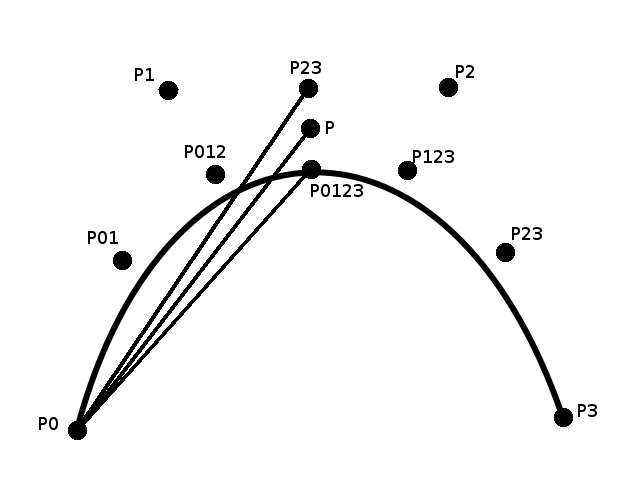
\includegraphics[scale=0.5]{bezier_pused}
\subsection{Drawing the glyph}
The distance gradients in the distance field will only be drawn locally within a predefined distance from each outline. This creates a need to draw the glyph in the image before generating the distance field. If the glyph is not drawn before the distance gradients are drawn there will most certainly be parts of the glyph that have the outside color but is located on the inside of the glyph or vice versa. For example the middle of the 'I' might have the same color as pixels outside the glyph. This would lead to a hole in the middle of the 'I' when rendering it which is not desired. The input to this step of the distance field generation is a glyph represented as connected line segments in the shape of a polygon. As mentioned in the background the scan-line algorithm together with the odd even fill rule or the non-zero winding rule can be used to fill a polygon. Because this is a very common problem in computer graphics and there are many open source libraries doing this very fast and optimized there were no need to implement this. The function drawPath in the open source 2D graphics library Skia was used instead. The Skia library was already installed and used in other places within Visiarc's products.
\subsection{Drawing distance gradients}
When drawing gradients it is convenient to draw them in primitive shapes like rectangles or triangles. To be able to draw gradients contiuously over the outline of the whole glyph two different distance gradients has to be drawn for each line segment. The first gradient is a rectangular gradient and the second gradient is a triangular gradient. The gradients are illustrated in figure \ref{fig:grad}.

\begin{figure}[H]
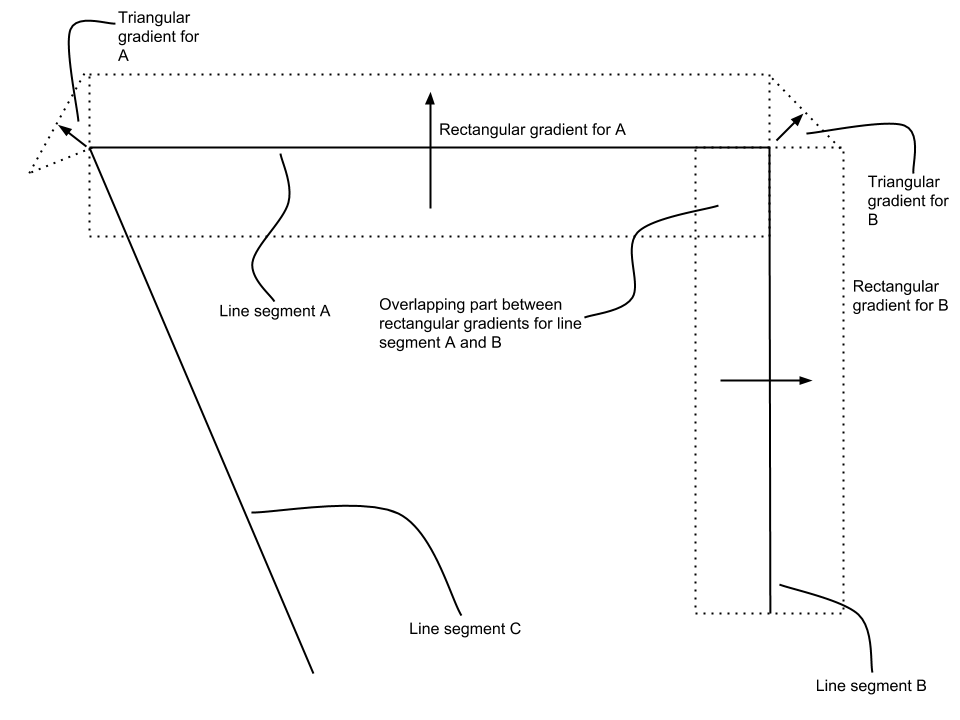
\includegraphics[scale=0.35]{gradient_drawing}
\caption{Line segment to pixel distance}
\label{fig:grad}
\end{figure}

The gradients are drawn in the direction of the arrows in the range from 0 to 255. This will make the inside of the glyph black/grey and the outside of the glyph white/grey. Because the glyph is drawn in the image using the Skia library before drawing the gradients there is no need for the gradients to cover the whole glyph. The triangular gradients are used to repair the distance field when two line segments are not parallel which is almost always the case. As illustrated in the figure it might occur problems in some areas when drawing the gradients. One of the problem areas is the overlap between different gradients. Another problem that might occur is that parts of gradients that should be on the inside of the glyph ends up on the outside or vice versa. This will happen if the angle between two line segments is less than 90 degrees. To solve both the mentioned problems a control is done before drawing in a pixel. A description of the control done follows. If the new and the old value are not both inside values or outside values do not draw. If both the new and the old value are inside values draw if and only if the old value is lower than the new value. If both the new and the old value are outside values, draw if and only if the old value is higher than the new value.

Drawing gradients can be done in many different ways. The initial implementation of this step in this thesis had real measured distances as values in each pixel in the gradient. The pixel to line segment distance was calculated by projecting the pixel coordinate onto the line. If the projection hit the line segment the distance was equal to the projection distance. Otherwise the distance was equal to the shortest distance to one of the endpoints of the line segment.

\begin{figure}[H]
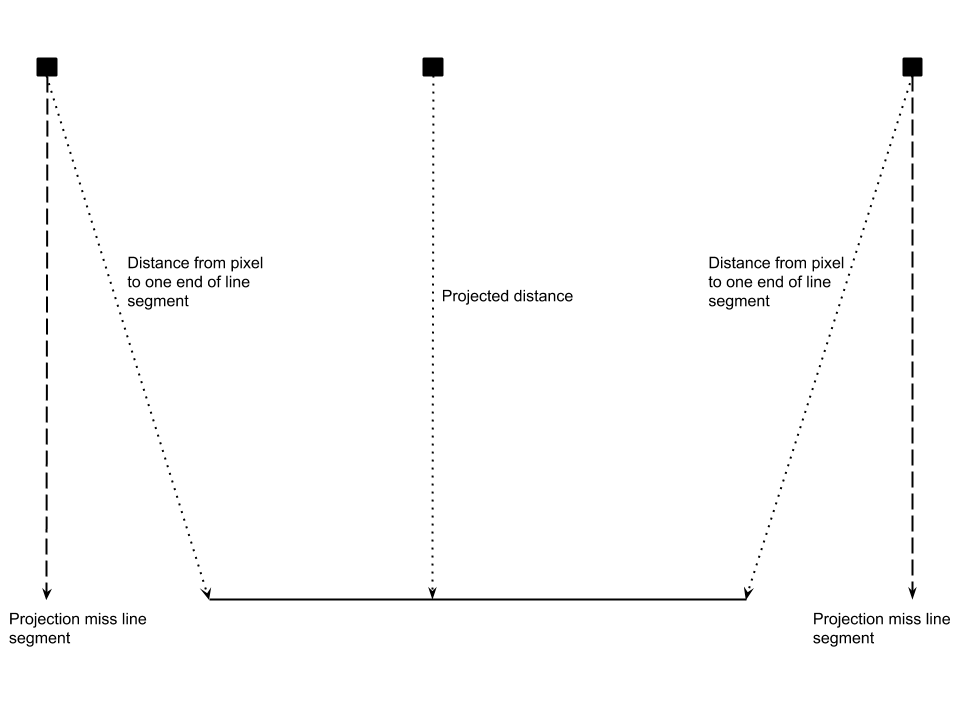
\includegraphics[scale=0.35]{pixel_line_measure}
\caption{Line segment to pixel distance}
\end{figure}

The code for projecting a pixel to a line segment made the distance fields look good because there was few sources of errors drawing the gradients. Every pixel was calculated independently from eachother and if the new distance was not better than the distance already in the pixel the pixel was not updated. The only problem with this approach was the execution time. The code for pixel to line segment distance calculation was located in the innermost loop which means that the code was executed very many times and performance improvements were neccessary.

In the distance field generation made by Qt no pixel to line projection is done. The rectangular gradients are drawn directly using trigonometric calculations stepping through the pixels row by row. This influenced how the rectangular gradients are drawn in the final result of this thesis. The problem by using this solution is to find the distance d in figure \ref{fig:distanced}.

\begin{figure}[H]
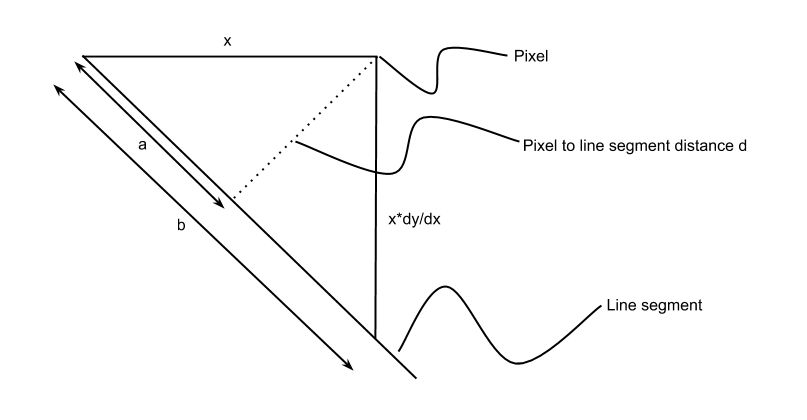
\includegraphics[scale=0.5]{draw_gradient}
\caption{Illustration of the calculations done when drawing the rectangular gradients}
\label{fig:distanced}
\end{figure}

The line segment is defined between two points in the plane $p_1$ and $p_2$. The derivative of the line can trivially be calculated $\frac{dy}{dx}=\frac{p_{2y}-p_{1y}}{p_{2x}-p_{1x}}$. The projection of the pixel to the line segment will always be perpendicular to the line segment which implies that the triangle with sides $x$, $x\frac{dy}{dx}$ and $b$ and the triangle with sides $x$, $a$ and $d$ are similar triangles. Similarity between two triangles means that the sides of the first triangle are proportional with the same constant to the sides of the second triangle. In mathematic terms it implies that $\frac{x}{b}=\frac{a}{x\frac{dy}{dx}}=\frac{d}{x}$ is true. The similarity of the triangles gives two ways to calculate $d$, either $d=\frac{x^2}{b}$ or $d=\frac{a}{\frac{dy}{dx}}$. The first solution is used in this thesis and b is calculated with the following formula $b=\sqrt{x^2+(x*\frac{dy}{dx})^2}$. Having $b$ the final formula for calculating d is $d=\frac{x^2}{\sqrt{x^2+(x*\frac{dy}{dx})^2}}=\frac{x}{\sqrt{1+\frac{dy}{dx}^2}}$. The shortest distance from the line segment to the pixel is equal to $|d|$.

The rectangular gradients are drawn by stepping through all the pixels covered by the rectangle row by row and calculating the distance d. The control mentioned previous in this section is used before drawing to remove the overlapping problems. Drawing the triangular gradients are done in the same way with one exception, that is the calculation of the distance d. The closest point on the line segment to the pixel in the triangular gradient will always be the corresponding endpoint p of the line segment closest to the triangular gradient. This makes it possible to calculate d as the distance from the pixel to the point p.

\section{Distance field rendering}
Distance field rendering is not as easy as usual image rendering. When rendering images to the screen with OpenGL the image is loaded into a texture and uploaded to the GPU. On the GPU the image is resized and interpolated to fit the pixels on the screen before it is drawn. The interpolation is a built in operation on the GPU. An image can be drawn to the screen with a basic vertex and fragment shader where the vertex shader pass through the coordinates of the polygon that the texture is mapped to and the fragment shader fetch the color corresponding to its pixel from the texture and output it to the screen. When rendering distance field glyphs a more complex fragment shader has to be used.

The basic idea with distance field rendering is that the interpolation of a greyscale image does not decrease quality of the glyph border as much as if the image was not a greyscale image. This will let the GPU interpolate the image to the screen preserving the information about where the outlines of the glyph are located before the fragment shader takes the decision whether the corresponding pixel is inside or outside the glyph. The most basic fragment shader for rendering distance field will set the output pixel transparent if the corresponding lookup in the distance field has a value greater or equal to $0.5$. On the GPU the color values are floats between 0 and 1 which means that outlines of the glyph are located at 0.5. This solution is really easy to implement and can be written as one line of code but it will create aliasing artifacts around the border of the glyph. To render good looking text using distance fields some kind of anti-aliasing is needed. 

A commonly used function when rendering distance field glyphs is the smoothstep function. The smoothstep function is a built in function in GLSL and it performs a smooth hermite interpolation between 0 and 1 in a range for an input value. The range and the value is parameters to the function. Using this function over an interval around the outline of the glyph will create a smoother edge and decrease the aliasing. This is a pretty cheap way to create descent anti-aliasing which can be modified when changing the interval. A bigger interval for example $[0.4,0.5]$ will create very blured edge while a smaller interval for example $[0.49,0.51]$ will create a sharper edge with the cost off possible aliasing effects. The smoothstep function is not enough aliasing reduction in many cases. There are methods to improve the anti-aliasing. One way used by \citet{gustavson20122d} is to use the glsl functions dFdx and dFdy which returns the derivatives of the distance field for the current pixel in the x and y axis. The function used in the fragment shader used in the article follows.
\begin{algorithm}[H]
\caption{Anti-aliasing function proposed by Gustavson}
\begin{algorithmic}
\Procedure{aastep}{float threshold, float distance}
\State float afwidth = 0.7 * length(vec2(dFdx(distance), dFdy(distance)));
\State \Return \Call{smoothstep}{threshold - afwidth, threshold + afwidth, distance};
\EndProcedure
\end{algorithmic}
\end{algorithm}
All three of the above described fragment shaders wer implemented in this thesis. Implementing all three makes it possible to choose shader depending on the computational power of the GPU. The first mentioned implementation with a simple threshold check is the fastest one and the last mentioned shader containing the aastep function is the slowest.
\subsection{Glyph positioning}

\chapter{Methods for evaluation of the implementation}
The goal with this thesis was to solve the problem formulation described in the introduction. To be able to evaluate if the goals wer achieved three different methods of evaluation were needed. The methods of evaluation are described in this chapter.
\section{Visual evaluation \#1}
Evaluating the visual appearance of rendered text is hard. The evaluation should be done in a way that it is justified to say that the text rendered with the implementation from this thesis is at least as good looking as the text rendered by the old implementation. One way to evaluate this is letting one or several persons judge if the text rendered with the new implementation is good enough. This method could be used in this thesis and the judge in this case would have been VisiArc which is the company this thesis is written for. The results from using this evaluation method would not be facts, it would be one or several personal oppinions. Because people have different oppinions this test could not be replicated by other people which is desirable. This is the reason this method was not used in this thesis.

To get a test that could be replicated a more technical test was needed. The method used for the first visual evaluation of glyphs rendered with the implementation from this thesis follows. Two equally big glyphs were rendered from both the old text implementation and from the new implementation from this thesis. This made it possible to compare pixel values between the two images and output a result. The result from the test was a greyscale image with the same size as the input images where white symbolizes difference and black no difference between the input images. The value for pixel n in the output image was calculated by taking the positive difference between pixel n in the first and the second image. In the output image it is easy to see where the errors are located and how big the errors are.
\section{Visual evaluation \#2} 
The second visual evaluation uses the same method as the first but output a different result. The output from this evaluation is a percentage of how many pixels is equal between the images. 
\section{Performance evaluation}
There are many ways to measure performance. Because a goal with this thesis was to be able to render text in real time a good measure for performance is the distance field generation speed. The distance field generation speed was measured as the time between the function call and the function return of the function generating distance field. The impact of different scheduling in the the mobile device CPU was neglected.
